% Theme ────────────────────────────────────────────────────────────────────────
\documentclass{settings/laserbeam}
\usepackage{media9} % For animations
\graphicspath{{./images/}} % Specifies the directory where pictures are stored

% Other stuff
\newcommand{\grayitem}{\item[\gray{$\bullet$}]}

% Title Slide ──────────────────────────────────────────────────────────────────
\title{
	\bft{Adaptive time-stepping for Navier-Stokes}
}
\subtitle{\small{
	Advanced Topics in Scientific Computing Course Final Project\\
	SDIC Master Degree, University of Trieste (UniTS) and SISSA
}}
\date{January 2025}
\titlegraphic{
	\begin{center}
    \begin{minipage}{0.45\textwidth}
        \begin{center}
		
\includegraphics[width=0.4\textwidth]{sdic-logo.png}
        \end{center}
    \end{minipage}
	\end{center}
}
\author{Piero Zappi}

% Slides ───────────────────────────────────────────────────────────────────────
\begin{document}

\frame{\titlepage} % This creates the title slide

\section{Presentation Outline}

\begin{frame}

	\frametitle{Presentation Outline}

	\vspace{-1.0cm}
	\begin{cbox}
		\begin{center}
			\itt{Adaptive time-stepping for solving the incompressible\\
            Navier-Stokes equations with a finite element method\\
             using the deal.II library}
		\end{center}
	\end{cbox}

	\begin{enumerate}
		\item \bft{Introduction}
		\item \bft{Adaptive Time-Stepping Algorithms}
			\begin{itemize}
				\grayitem \gray{First Approach}
				\grayitem \gray{Second Approach (\itt{chosen one})}
			\end{itemize}
		\item \bft{Results}
		\item \bft{Conclusions}
	\end{enumerate}

\end{frame}

\section{Introduction}

\begin{frame}
	\begin{cbox}
		{\fontsize{20pt}{7.2}\selectfont \bft{Introduction}}
	\end{cbox}
\end{frame}

\begin{frame}
    
    \frametitle{Adaptive Time-Stepping}

    \begin{cbox}
    \begin{itemize}
        \item \textbf{Purpose:} control \itt{accuracy} and reduce \itt{computational costs}.
        \item \textbf{Key Idea:} dynamically adjust time step size based on error estimators:
        \begin{itemize}
            \item \textbf{Increase} time step size when error is small (\itt{efficiency}).
            \item \textbf{Decrease} time step size when error is large (\itt{accuracy}).
        \end{itemize}
        \item \textbf{Challenges with Fixed Time-Stepping:}
        \begin{itemize}
            \item Too small time steps $\rightarrow$ \itt{waste of computational resources}.
            \item Too large time steps $\rightarrow$ \itt{leads to inaccurate solutions}.
        \end{itemize}
        \item \textbf{Goal:} find the \itt{optimal time step size} at each time step, following the time evolution of the \itt{physics} of the flow.
    \end{itemize}
    \end{cbox}

\end{frame}

\begin{frame}
    
    \frametitle{Project Development Overview}

    \begin{cbox}
    \begin{itemize}
        \item \textbf{Foundation:} based on \textbf{Step-35 tutorial} of the deal.II library.
        \begin{itemize}
            \item Solves \itt{incompressible, time-dependent Navier-Stokes equations} using a \textbf{projection method} (decouples velocity and pressure).
        \end{itemize}
    \end{itemize}
    \end{cbox}
    \vspace{0.5cm}
    \begin{cbox}
    \begin{itemize}
        \item \textbf{Enhancement:}
        \begin{itemize}
            \item Original program uses \textbf{fixed time steps}.
            \item Extended to implement \textbf{adaptive time-stepping}:
            \begin{itemize}
                \item \textbf{Dynamic adjustment} of time step size via error estimators.
                \item Improves simulation \textbf{efficiency} and \textbf{accuracy}.
            \end{itemize}
        \end{itemize}
    \end{itemize}
    \end{cbox}

\end{frame}

\section{Adaptive Time-Stepping Algorithms}

\begin{frame}
	\begin{cbox}
		{\fontsize{20pt}{7.2}\selectfont \bft{Adaptive Time-Stepping\\ Algorithms}}
	\end{cbox}
\end{frame}

\begin{frame}
    
    \frametitle{First Approach - Main Concepts}

    \begin{cbox}
    \begin{itemize}
        \item \textbf{Overview}:
        \begin{itemize}
            \item Based on \textbf{two solutions} computed with schemes of \textbf{different orders of accuracy}.
            \item \textbf{Key Idea}: use the difference between the solutions to estimate the next time step size.
        \end{itemize}
    \end{itemize}
    \end{cbox}
\end{frame}

\begin{frame}
    
    \frametitle{Error Estimation and Optimal Time Step Size}

    \begin{cbox}
    \begin{itemize}
        \item \textbf{Error Estimation}:
        \begin{itemize}
            \item $u$: less accurate solution, error $\mathcal{O}(\Delta t^p)$.
            \item $\bar{u}$: more accurate solution, error $\mathcal{O}(\Delta t^{p+1})$.
            \item Difference between solutions:
            $$
            e = ||\bar{u}-u||_{L^2} \approx C \Delta t^p
            $$
        \end{itemize}
    \end{itemize}
    \end{cbox}
    \vspace{0.5cm}
    \begin{cbox}
    \begin{itemize}
        \item \textbf{Optimal Time Step Size} ($\Delta t_{\text{opt}}$):
        \begin{itemize}
            \item Given tolerance $\epsilon>0$.
            \item $\rho$: safety factor ($0<\rho\leq1$).
            \item Compute:
            $$
            \Delta t_{\text{opt}} = \rho \Delta t \left( \frac{\epsilon}{e} \right)^{1/p}
            $$
        \end{itemize}
    \end{itemize}
    \end{cbox}
\end{frame}

\begin{frame}
    
    \frametitle{Drawbacks of the First Approach}

    \begin{cbox}
    \begin{itemize}
        \item \textbf{High computational cost}:
        \begin{itemize}
            \item Requires \textbf{two solutions} with different schemes.
            \item \textbf{Doubles the cost of the simulation}.
        \end{itemize}
    \end{itemize}
    \end{cbox}
    \vspace{0.5cm}
    \begin{warning}
        Inefficiency may nullify the benefits of adaptive time-stepping.
    \end{warning}
\end{frame}

\begin{frame}

    \frametitle{Second Approach - Main Concepts}

    \begin{cbox}
    \begin{itemize}
        \item \textbf{Overview}:
        \begin{itemize}
            \item More \textbf{efficient} than the first approach: only \textbf{one solution} is used (\gray{\itt{projection method}}).
            \item Adjusts time step size based on the \textbf{relative change in the solution over two consecutive time steps}.
            \item Dynamically adapts to the \textbf{physics} of the flow.
            \item The time step size is reduced when the system is evolving rapidly, it is increased when the system is evolving slowly.
        \end{itemize}
    \end{itemize}
    \end{cbox}
    \vspace{0.5cm}
    \begin{blueinfo}
        This approach is the one implemented in the project.
    \end{blueinfo}
\end{frame}

\begin{frame}

    \frametitle{Time Error Indicator}

    \begin{cbox}
    \textbf{Error Quantification}:
    \begin{itemize}
        \item Measures relative change in the solution using:
        $$
        (\eta^n)^2 = \sum_{K\in T_h} \left( \int_{t^{n-1}}^{t^n} \left(||\nabla\left(u_h^{n}-u_h^{n-1}\right)||^2_{L^2(K)}\right)dt \right)
        $$
        \begin{itemize}
            \item $T_h$: mesh.
            \item $u_h^{n}$, $u_h^{n-1}$: solutions at $t^n, t^{n-1}$.
        \end{itemize}
    \end{itemize}
    \textbf{Normalization term}:
    $$
    (\sigma^n)^2 = \int_{t^{n-1}}^{t^n} |u_h^{n}|^2_{1}dt
    $$
    \begin{itemize}
        \item $|u_h^{n}|_{1}$: $H^1$ semi-norm of the solution.
    \end{itemize}
    \end{cbox}
\end{frame}

\begin{frame}
    
    \frametitle{Optimal Time Step Size}

    \begin{cbox}
    \textbf{Bound on Time Error Indicator}:
    $$
    (1-\alpha)\text{TOL}\leq\frac{\eta^n}{\sigma^n}\leq(1+\alpha)\text{TOL}
    $$
    \begin{itemize}
        \item $\text{TOL}=0.1$: tolerance.
        \item $\alpha=0.5$.
    \end{itemize}
    \end{cbox}
\end{frame}

\begin{frame}
    
    \frametitle{Optimal Time Step Size}

    \begin{cbox}
    \textbf{Adjustment Rules}:
    \begin{itemize}
        \item If bounds are \textbf{satisfied}:
        $$
        \Delta t_{\text{opt}} = \Delta t^n
        $$
        \item If $(\eta^n)^2 > (\sigma^n)^2(1+\alpha)^2\text{TOL}^2$:
        $$
        \Delta t_{\text{opt}} = \frac{\Delta t^n}{\rho_1}\quad\text{with}\quad\rho_1 =  \text{min}\left(\frac{(\eta^n)^2}{(\sigma^n)(1+\frac{\alpha}{2})^2\text{TOL}^2},2\right)
        $$
        \item If $(\eta^n)^2 < (\sigma^n)^2(1-\alpha)^2\text{TOL}^2$:
        $$
        \Delta t_{\text{opt}} = \frac{\Delta t^n}{\rho_2}\quad\text{with}\quad\rho_2 =  \text{max}\left(\frac{(\eta^n)^2}{(\sigma^n)(1-\frac{\alpha}{2})^2\text{TOL}^2},0.5\right)
        $$
        \end{itemize}
    \end{cbox}
\end{frame}

\begin{frame}
    
    \frametitle{Optimal Time Step Size}

    \begin{info}
        \textbf{Stability Constraints}:
        \begin{itemize}
            \item Choice of $\rho_1$ and $\rho_2$ ensures no \textbf{large variations} in the time step size, preventing \textbf{instabilities} in simulations.
            \item \textbf{Bounded time step size}:
            $$
            \Delta t_{\text{min}}=10^{-4}\quad\text{and}\quad\Delta t_{\text{max}}=0.1
            $$
            \end{itemize}
    \end{info}
\end{frame}

\section{Results}

\begin{frame}
	\begin{cbox}
		{\fontsize{20pt}{7.2}\selectfont \bft{Results}}
	\end{cbox}
\end{frame}

\begin{frame}
    
    \frametitle{Test Case: Flow Around a Square Obstacle}

    \begin{itemize}
    \item \textbf{Geometry}:
    \begin{center}
        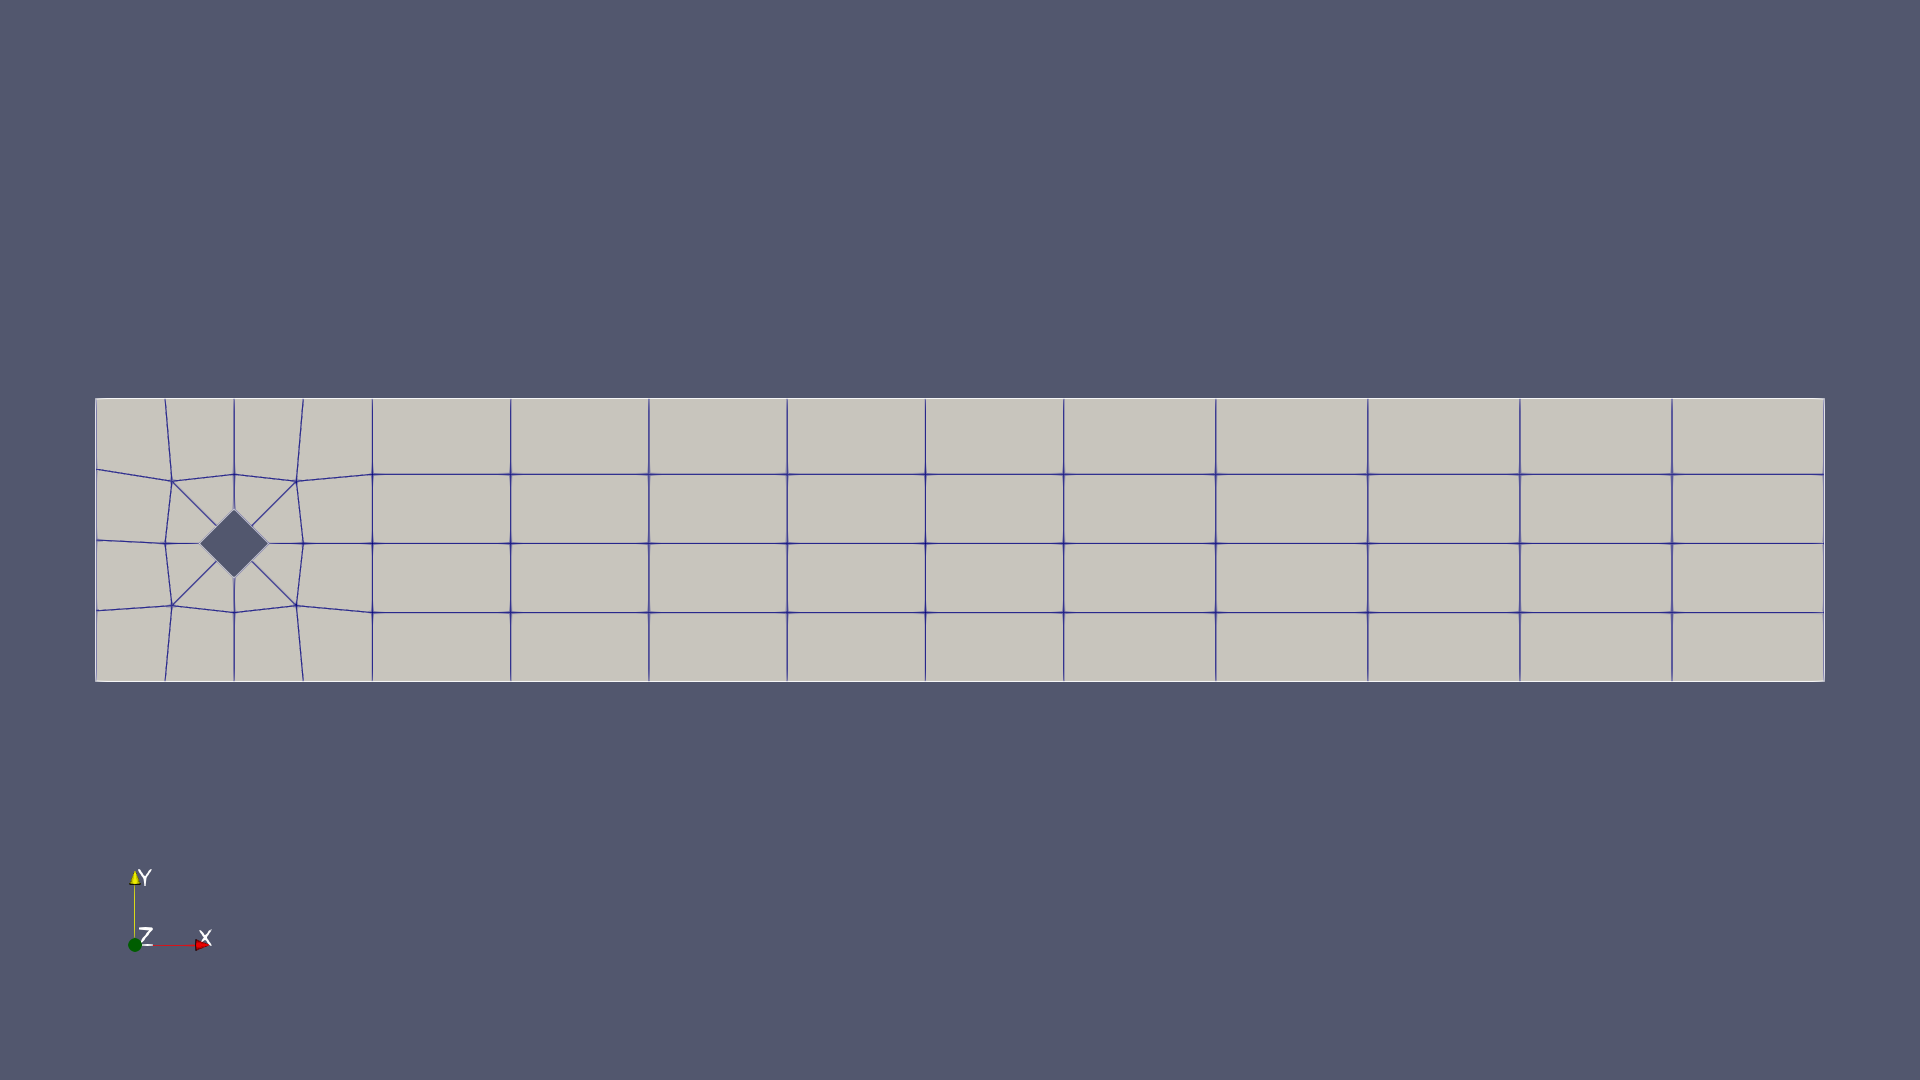
\includegraphics[width=0.5\textwidth]{images/test_geometry.png}
    \end{center}
    \item \textbf{Boundary Conditions}:
    \begin{itemize}
        \item \textbf{No-slip}: top/bottom walls and the obstacle.
        \item \textbf{Inflow} (left wall):
        $$
        u = \begin{cases}
            4U_my\frac{(H-y)}{H^2} \\
            0
        \end{cases}
        $$
        \begin{itemize}
            \item $U_m=1.5$, $H=4.1$.
        \end{itemize}
        \item \textbf{Outflow} (right wall):
        \begin{itemize}
            \item Vertical velocity component is set to zero.
            \item Pressure is set to zero.
        \end{itemize}
    \end{itemize}
    \end{itemize}
    
\end{frame}

\begin{frame}
    
    \frametitle{Mesh Refinement Levels}

    \begin{cbox}
    \begin{itemize}
        \item \textbf{Meshes Used}:
        \begin{itemize}
            \item \itt{Level 1} mesh (\itt{coarser}), $960$ cells. \gray{\itt{2 refinement levels}}.
            \item \itt{Level 2} mesh (\itt{finer}), $3840$ cells. \gray{\itt{3 refinement levels}}.
        \end{itemize}
    \end{itemize}
    \end{cbox}
    \vspace{0.2cm}
    \begin{center}
        \begin{figure}[H]
            \begin{minipage}{0.4\linewidth}
                \begin{center}
                   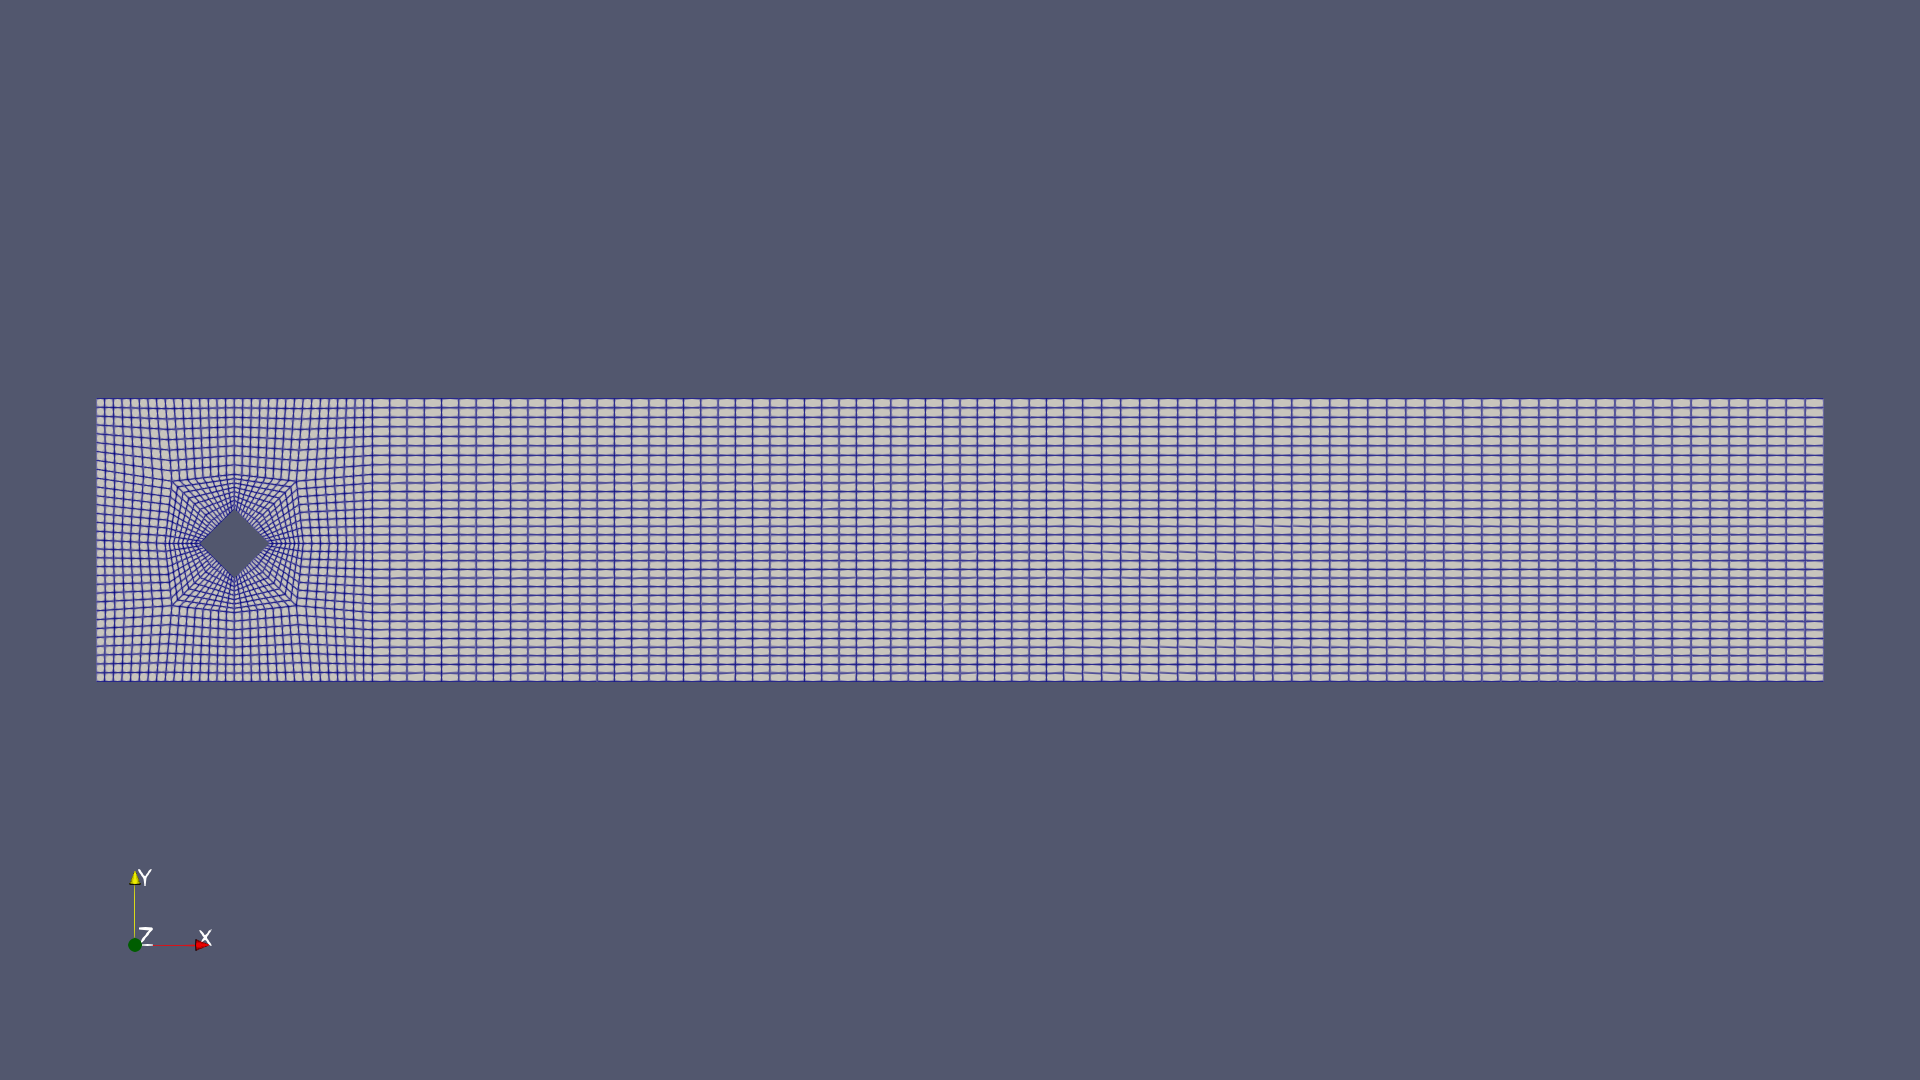
\includegraphics[width=1\linewidth]{images/2_ref_levels.png}
                   \caption{Level 1 mesh}
                \end{center}
            \end{minipage}
            \qquad
            \qquad
            \begin{minipage}{0.4\linewidth}
                \begin{center}
                    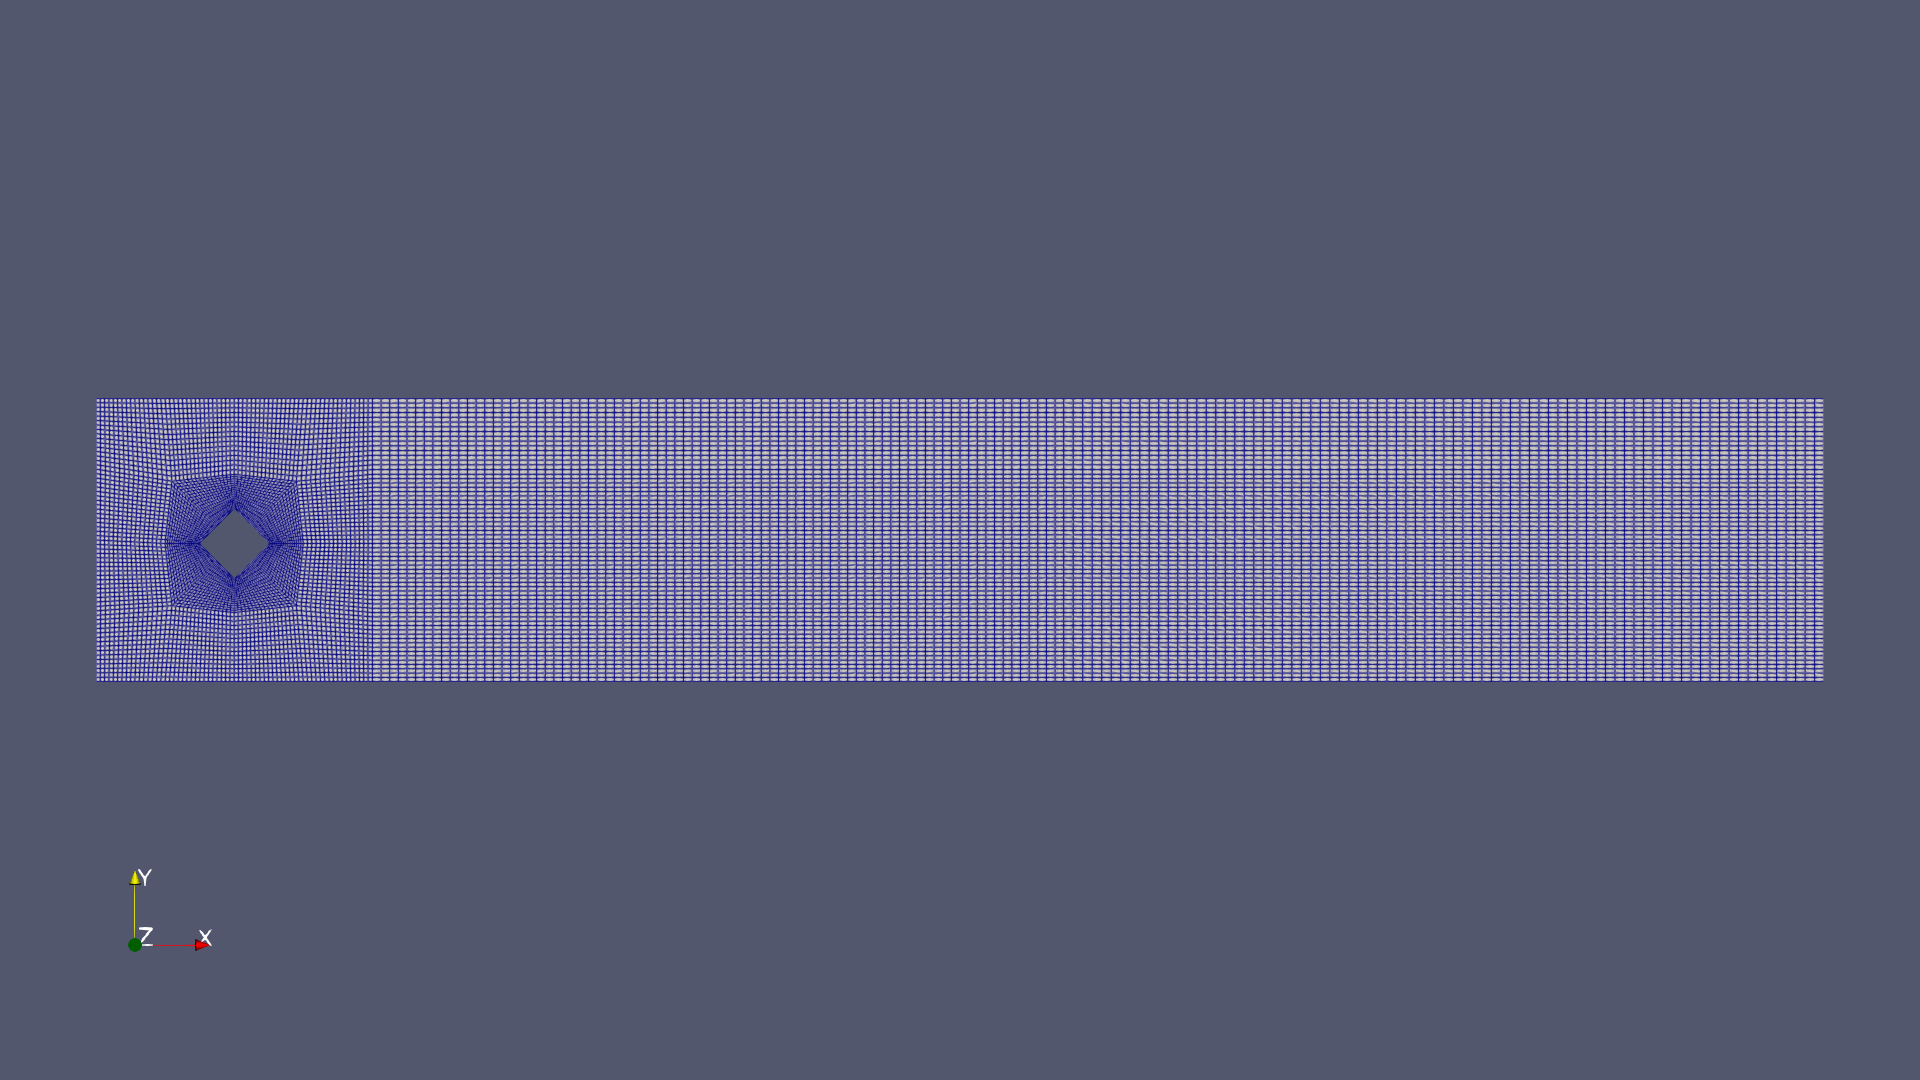
\includegraphics[width=1\linewidth]{images/3_ref_levels.png}
                    \caption{Level 2 mesh}
                \end{center}
            \end{minipage}
        \end{figure}
    \end{center}

\end{frame}

\begin{frame}
    
    \frametitle{Parameter Settings}

    \begin{cbox}
    \textbf{Reynolds Numbers}:
    \begin{itemize}
        \item Simulations performed for:
        $$
        \text{Re} = 50, 100, 200
        $$
    \end{itemize}
    \end{cbox}
    \vspace{0.5cm}
    \begin{cbox}
    \textbf{Time and Output Settings}:
    \begin{itemize}
        \item Final simulation time: $T=40$.
        \item Initial time step size: $\Delta t_0=0.001$.
        \item Output interval: every $20$ time steps.
    \end{itemize}
    \end{cbox}

\end{frame}

\begin{frame}
    
    \frametitle{Simulation Results}

    \begin{cbox}
        \textbf{Case:} \itt{level 2} mesh, \itt{Re} $= 100$.
    \end{cbox}
    \vspace{0.2cm}
    \begin{center}
        \begin{figure}[H]
            \begin{minipage}{0.4\linewidth}
                \begin{center}
                    \includemedia[
                        width=1\linewidth,
                        height=0.55\linewidth,
                        activate=onclick,
                        passcontext,  % Ensures it works for all viewers
                        addresource=images/sol.mp4,
                        flashvars={
                            source=images/sol.mp4
                            &loop=true
                            &autoplay=true
                        }
                    ]{}{VPlayer.swf}
                \end{center}
            \end{minipage}
            \qquad
            \qquad
            \begin{minipage}{0.4\linewidth}
                \begin{center}
                    \includemedia[
                        width=1\linewidth,
                        height=0.55\linewidth,
                        activate=onclick,
                        passcontext,  % Ensures it works for all viewers
                        addresource=images/sol_LIC.mp4,
                        flashvars={
                            source=images/sol_LIC.mp4
                            &loop=true
                            &autoplay=true
                        }
                    ]{}{VPlayer.swf}
                \end{center}
            \end{minipage}
        \end{figure}
    \end{center}
    \vspace{0.2cm}
    \begin{cbox}
        Animations show the development and extension of a vortex chain behind the obstacle, with formation and shedding of vortices downstream.
    \end{cbox}

\end{frame}

\begin{frame}
    
    \frametitle{Adaptive Time-Stepping Analysis}

    \begin{center}
        \begin{figure}[H]
            \begin{minipage}{0.43\linewidth}
                \begin{center}
                   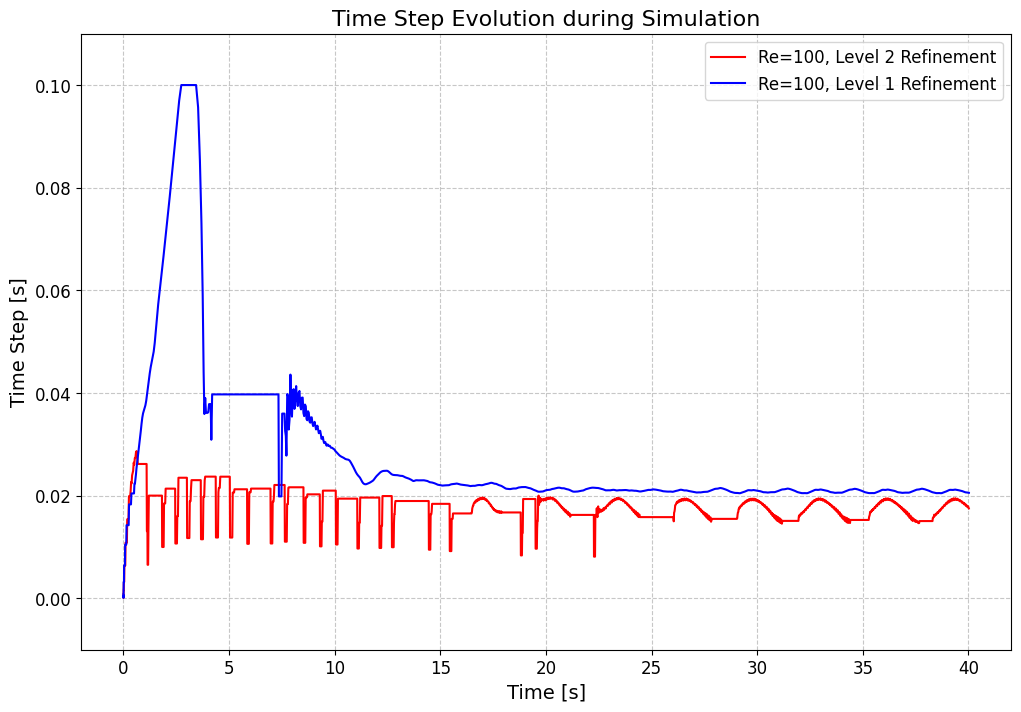
\includegraphics[width=1\linewidth]{images/Ref_Level_Comp.png}
                \end{center}
            \end{minipage}
            \qquad
            \qquad
            \begin{minipage}{0.43\linewidth}
                \begin{center}
                    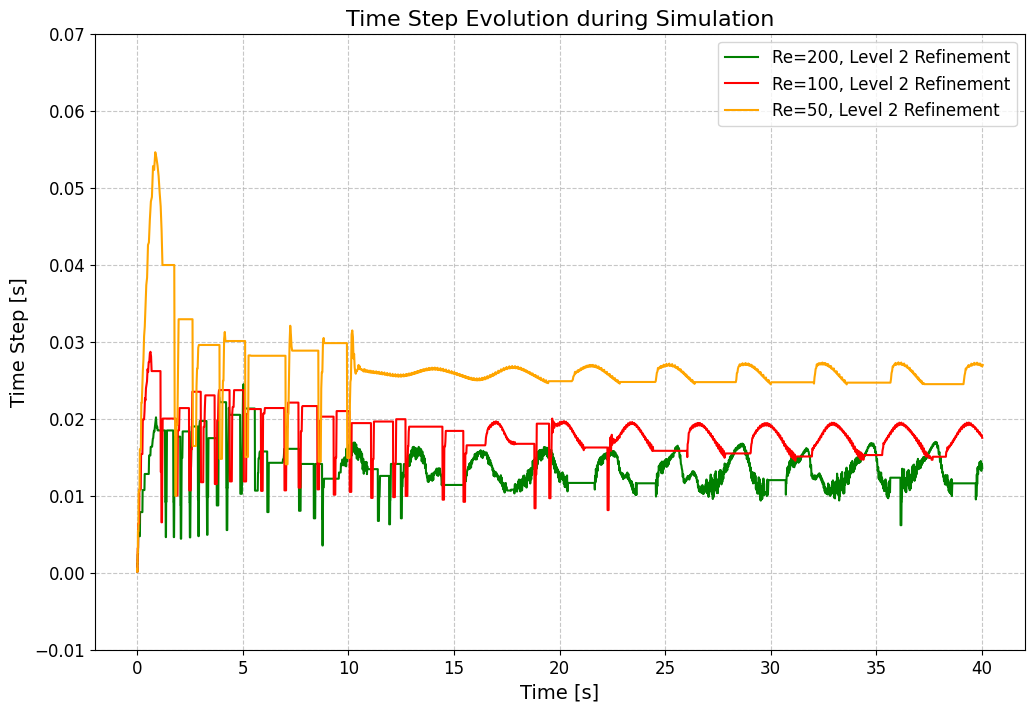
\includegraphics[width=1\linewidth]{images/Re_Comp.png}
                \end{center}
            \end{minipage}
        \end{figure}
    \end{center}
    \only<1>{
    \begin{cbox}
        \textbf{General Trends}:
        \begin{enumerate}
            \item \textbf{Initialization phase}: time step size decreases.
            \item \textbf{Stabilization phase}: time step size increases.
            \item \textbf{Vortex Shedding phase}: time step size oscillates.
            \item \textbf{Periodic phase}: time step size stabilizes achieving a periodic trend.
        \end{enumerate}
    \end{cbox}}
    \only<2>{
    \begin{cbox}
        \textbf{Effect of the Grid Refinement}:
        \begin{enumerate}
            \item \itt{Level 2 Mesh (Finer Grid)}:
            \begin{itemize}
                \item Smaller time step sizes.
                \item Increased sensitivity to the flow dynamics.
                \item More oscillatory behavior.
            \end{itemize}
            \item \itt{Level 1 Mesh (Coarser Grid)}:
            \begin{itemize}
                \item Larger time step sizes.
                \item Reduced sensitivity to the flow dynamics.
                \item Smoother trend.
            \end{itemize}
        \end{enumerate}
    \end{cbox}}
    \only<3>{
    \begin{cbox}
        \textbf{Effect of the Reynolds Number}:
        \begin{enumerate}
            \item \itt{Higher Reynolds Numbers}:
            \begin{itemize}
                \item Smaller time step sizes.
                \item Increased oscillatory behavior
            \end{itemize}
            \item \itt{Lower Reynolds Numbers}:
            \begin{itemize}
                \item Larger time step sizes.
                \item Reduced oscillations.
            \end{itemize}
        \end{enumerate}
    \end{cbox}}

\end{frame}

\begin{frame}
    
    \frametitle{Effectiveness of the Adaptive Time-Stepping Algorithm}

    \only<1>{
    \begin{cbox}
        \begin{enumerate}
            \item \textbf{Dynamic Time Step Adjustment}:
            \begin{itemize}
                \item Time step size is \textbf{reduced} during:
                \begin{itemize}
                    \item Rapid solution evolution.
                    \item Formation of flow structures and vortices.
                \end{itemize}
                \item Time step size is \textbf{increased} during:
                \begin{itemize}
                    \item Stabilization of the flow.
                    \item Reduced solution variability.
                \end{itemize}
            \end{itemize}
            \item \textbf{Optimized Computational Efficiency}:
            \begin{itemize}
                \item Balances \textbf{accuracy} and \textbf{efficiency} dynamically.
            \end{itemize}
        \end{enumerate}
    \end{cbox}}
    \only<2>{
    \begin{cbox}
        \textbf{Alignment with Expected Trends}:
        \begin{itemize}
            \item \itt{Finer Grid Refinements}:
            \begin{itemize}
                \item Smaller time step sizes required to resolve detailed flow structures.
            \end{itemize}
            \item \itt{Higher Reynolds Numbers}:
            \begin{itemize}
                \item Smaller and more oscillatory time steps to capture faster dynamics.
            \end{itemize}
        \end{itemize}
    \end{cbox}}

\end{frame}

\section{Conclusions}

\begin{frame}
    \begin{cbox}
        {\fontsize{20pt}{7.2}\selectfont \bft{Conclusions}}
    \end{cbox}
\end{frame}

\begin{frame}
    
    \frametitle{Conclusions}

    \begin{cbox}
        The adaptive time-stepping algorithm performs as expected, adjusting time step sizes effectively to:
        \begin{itemize}
            \item Reflect the \textbf{time evolution} of the physical flow.
            \item Optimize \textbf{efficiency} without compromising \textbf{accuracy}.
        \end{itemize}
    \end{cbox}
    \vspace{0.1cm}
    \begin{info}
        The analysis of the computed time step size evolution can help to better identify different phases of the flow.
    \end{info}
    \vspace{0.1cm}
    \begin{cbox}
        \textbf{Possible Future Extension}:
        \begin{itemize}
            \item Add \itt{adaptive mesh refinement} to further enhance the simulation accuracy.
        \end{itemize}
    \end{cbox}

\end{frame}

\section{References}

\begin{frame}

    \frametitle{References}

	{\fontsize{8pt}{7.2}\selectfont

    [1] Step-35 tutorial program of the deal.II library: a projection solver for the Navier–Stokes equations.\\
    \vspace{1em}

    [2] Berrone, S. and Marro, M., 2009. Space–time adaptive simulations for unsteady Navier–Stokes problems. Computers & Fluids, 38(6), pp.1132-1144.\\
    \vspace{1em}

    [3] Kay, D.A., Gresho, P.M., Griffiths, D.F. and Silvester, D.J., 2010. Adaptive time-stepping for incompressible flow part II: Navier–Stokes equations. SIAM Journal on Scientific Computing, 32(1), pp.111-128.\\
    \vspace{1em}

    [4] Boisneault, A., Dubuis, S. and Picasso, M., 2023. An adaptive space-time algorithm for the incompressible Navier-Stokes equations. Journal of Computational Physics, 493, p.112457.\\
    \vspace{1em}

    [5] John, V. and Rang, J., 2010. Adaptive time step control for the incompressible Navier–Stokes equations. Computer Methods in Applied Mechanics and Engineering, 199(9-12), pp.514-524.\\
	}

\end{frame}

\end{document}